%Dạng 1
\setcounter{ex}{0}
\section{Phép đếm}
\subsection{Kiến thức cần nhớ}
\begin{khung}
	\subsubsection{Góc giữa đường thẳng và mặt phẳng}
	\immini{Muốn xác định góc của đường thẳng $a$ và $(P)$ ta tìm hình chiếu vuông góc $a'$ của $a$ trên $(P)$. Khi đó $\left(\widehat{a,(P)}\right)=\left(\widehat{a,a'}\right)$.}
	{\begin{tikzpicture}[scale=0.6, font=\footnotesize, line join=round, line cap=round, >=stealth]
		\tkzInit[ymin=-5,ymax=0.5,xmin=-4.1,xmax=4.1]
		\tkzClip 
		\tkzDefPoints{-4/-4/M, -2/-1.5/Q, 2/-4/N, -0.5/-3/H}
		\tkzDefPointBy[translation = from M to N](Q) \tkzGetPoint{P}
		\tkzDefLine[perpendicular=through H,K=0.4](Q,P) \tkzGetPoint{h}
		\tkzInterLL(H,h)(Q,P) \tkzGetPoint{h_1}
		\coordinate[label={above right}:$A$] (A) at ($(h_1)+(0,1)$);
		\tkzDefLine[parallel=through H](Q,P) \tkzGetPoint{x}
		\coordinate[label={above right}:$O$] (O) at ($(H)!0.4!(x)$);
		\tkzInterLL(A,O)(N,P) \tkzGetPoint{O_1}
		\tkzInterLL(A,O)(P,Q) \tkzGetPoint{O_3}
		\coordinate (O_2) at ($(O)!3.3!(O_1)$);
		\tkzLabelPoints[below](H)
		\tkzDrawLines[add=0 and 0.3](O,H O,A)
		\tkzDrawSegments[dashed](h_1,O_3 O,O_1)
		\tkzDrawSegments(M,N N,P P,O_3 h_1,Q Q,M A,H O_1,O_2)
		\tkzLabelLine[below left,pos=1.3](O,A){$a$}
		\tkzLabelLine[above,pos=1.3](O,H){$a'$}
		\tkzMarkRightAngle(A,H,O)
		\tkzMarkAngles[arc=l,size=0.7cm](A,O,H)
		\tkzLabelAngle[pos=0.9](A,O,H){$\varphi$}
		\tkzMarkAngles[arc=l,size=1.1cm](N,M,Q)
		\tkzLabelAngle[pos=0.7](N,M,Q){$\alpha$}
		\end{tikzpicture}
	}
	\subsubsection{Góc giữa hai mặt phẳng}
	\immini
		{Để tìm góc giữa hai mặt phẳng, đầu tiên tìm giao tuyến của hai mặt phẳng. Sau đó tìm hai đường thẳng lần lượt thuộc hai mặt phẳng cùng vuông góc với giao tuyến tại một điểm. Góc giữa hai mặt phẳng là góc giữa hai đường thẳng vừa tìm.}
		{
		\begin{tikzpicture}[scale=0.7, line join = round, line cap = round]
		\tkzDefPoints{0/0/A, 6/0/B, 4/3/C, -2/3/D,-2/-2/E,4/-2/F,2/0/G,0.5/-1.5/H,0.5/2/K}
		\tkzDrawSegments(B,C C,D D,A A,E E,F F,B G,H G,K)
		\tkzDrawSegments[dashed](A,B)
		\draw (3.8,3) node[below]{$Q$};
		\draw (-1.8,-1.8) node[right]{$P$};
		\draw (1,2) node{$d_1$};
		\draw (1,-1.5) node{$d_1$};
		\tkzMarkAngles(F,E,A)
		\tkzMarkAngles(D,C,B)
		\tkzMarkRightAngles(B,G,K)
		\tkzMarkRightAngles(H,G,A)
		\tkzMarkAngles(K,G,H)
		\end{tikzpicture}
			}
			\textbf{Những trường hợp đặc biệt dễ hay xảy ra$\colon$}
			\begin{enumerate}
				\item \underline{\textbf{Trường hợp $1\colon$}} Hai tam giác cân $ACD$ và $BCD$ có chung cạnh đáy $CD$, thì góc giữa hai mặt phẳng $(ACD)$ và $(BCD)$ là góc $\widehat{AHB}$.
				\begin{flushright}
					\begin{tikzpicture}[scale=0.7, line join = round, line cap = round]
					\tkzDefPoints{0/0/A,4/0/C,2/-2/D,3/-1/H}
					\coordinate (B) at ($(A)+(0,3)$);
					\tkzDrawSegments(B,D B,C A,D D,C B,H)
					\tkzDrawSegments[dashed](A,C A,H)
					\tkzDrawPoints[fill = black](A,D,C,B)
					\tkzLabelPoints[above](B)
					\tkzLabelPoints[below](D)
					\tkzLabelPoints[left](A)
					\tkzLabelPoints[right](C,H)
					\tkzMarkRightAngles(B,H,C)
					\tkzMarkRightAngles(A,H,D)
					\tkzMarkAngles(B,H,A)
					\tkzMarkSegments[mark=|](D,H C,H)
					\end{tikzpicture}
				\end{flushright}
				\item \underline{\textbf{Trường hợp $2\colon$}} Hai tam giác $ACD$ và $BCD$ bằng nhau có chung cạnh $CD$. Dựng $AH\perp CD \Rightarrow BH\perp CD$. Vậy góc giữa hai mặt phẳng $(ACD)$ và $(BCD)$ là góc $\widehat{AHB}$.
				\begin{flushright}
					\begin{tikzpicture}[scale=0.7, line join = round, line cap = round]
					\tkzDefPoints{0/0/B,4/0/D,2/-2/C,3/-1/H}
					\coordinate (A) at ($(B)+(2,3)$);
					\tkzDrawSegments(A,B A,C A,D A,H B,C C,D)
					\tkzDrawSegments[dashed](B,D B,H)
					\tkzDrawPoints[fill = black](A,B,C,D)
					\tkzLabelPoints[above](A)
					\tkzLabelPoints[below](C)
					\tkzLabelPoints[left](B)
					\tkzLabelPoints[right](H,D)
					\tkzMarkRightAngles(A,H,D)
					\tkzMarkRightAngles(B,H,C)
					\tkzMarkAngles(A,H,B)
					\end{tikzpicture}	
				\end{flushright}
				\item \underline{\textbf{Trương hợp $3\colon$}} Khi xác định góc giữa hai mặt phẳng khó quá, ta nên sử dụng công thức sau$\colon$
				$$\sin\varphi =\dfrac{d\left( A,mp(Q)\right)}{d(A,a)}$$
				Với $\varphi$ là góc giữa hai mặt phẳng $(P)$ và mặt phẳng $(Q)$, $A$ là một điểm thuộc mặt phẳng $(P)$ và $a$ là giao tuyến của hai mặt phẳng $(P)$ và $(Q)$.
				\item \underline{\textbf{Trường hợp $4\colon$}} Có thể tìm góc giữa hai mặt phẳng bằng công thức $S' = S.\cos\varphi$.
				\item \underline{\textbf{Trường hợp $5\colon$}} Tìm hai đường thẳng $d$ và $d'$ lần lượt vuông góc với mặt phẳng $(P)$ và mặt phẳng $(Q)$. Góc giữa hai mặt phẳng là góc giữa $d$ và $d'$.
				\item \underline{\textbf{Trường hợp $6\colon$}} Cách xác định góc giữa mặt phẳng bên và mặt phẳng đáy
				\begin{enumerate}
					\item Bước $1\colon$ Xác định giao tuyến $d$.
					\item Bước $2\colon$ Từ hình chiếu vuông góc của đỉnh, dựng $AH \perp d$.
					\item Bước $3\colon$ Góc cần tìm là góc $\widehat{SHA}$.\\
					Với $S$ là đỉnh, $A$ là hình chiếu vuông góc của đỉnh trên mặt đáy.
				\end{enumerate}
			\end{enumerate}
			\subsubsection{Khoảng cách từ một điểm đến mặt phẳng}
			\textbf{Bài toán 1. Tính khoảng cách từ hình chiếu vuông góc của đỉnh đến một mặt bên}\\
			Phương pháp xác định khoảng cách từ hình chiếu của đỉnh đến một mặt phẳng bên.
			\begin{center}
				\begin{tikzpicture}	[scale=.7, font=\footnotesize, line join=round, line cap=round, >=stealth]
				\coordinate (A) at (0,0);
				\coordinate (S) at (0,5);
				\coordinate (B) at (2,-2);
				\coordinate (C) at (6,0);
				\coordinate (H) at ($(B)!.55!(C)$);
				\coordinate (I) at ($(S)!.4!(H)$);
				\draw (S)--(A)--(B)--(C)--(S)--(B) (S)--(H);
				\draw[dashed] (H)--(A)--(C) (A)--(I);
				\tkzMarkRightAngle(A,H,B)
				\tkzMarkRightAngle(S,H,C)
				\tkzMarkRightAngle(A,I,H)
				\foreach \p/\pos in {S/above, A/left, B/below, C/right, H/below right, I/above right}
				\fill (\p) circle (1pt) node[\pos] {$\p$};
				\end{tikzpicture}
			\end{center}
			\begin{itemize}
				\item \textbf{Bước 1.} Xác định giao tuyến $\Delta$.
				\item \textbf{Bước 2.} Từ hình chiếu vuông góc của đỉnh, dựng $AH\perp \Delta$ (với $H\in \Delta$).
				\item \textbf{Bước 3.} Dựng $AI\perp SH$ (với $I\in SH$). Khoảng cách cần tìm là $AI$.\\
				Với $S$ là đỉnh, $A$ là hình chiếu vuông góc của đỉnh trên mặt đáy. 
				\item \textbf{Bước 4.} $ AI=\dfrac{SA\cdot AH}{\sqrt{SA^2+AH^2}} $
			\end{itemize} 
			Ba bước dựng ở trên là sử dụng tính chất: Hai mặt phẳng vuông góc với nhau, nếu một đường thẳng nằm trên mặt phẳng này vuông góc với giao tuyến thì sẽ vuông góc với mặt phẳng kia.\\
			\textit{Đây là bài toán cơ bản nhưng vô cùng quan trọng trong việc tính khoảng cách từ một điểm đến một mặt phẳng. Hầu như tính khoảng cách từ một điểm bất kì đến mặt phẳng bên đều thông qua điểm này dựa vào công thức của Bài toán 2}.\\
			
			\noindent \textbf{Bài toán 2. Tính khoảng cách từ một điểm bất kỳ đến một mặt phẳng}\\
			Thường sử dụng công thức sau:
			\begin{center}
				\begin{tikzpicture}	[scale=1, font=\footnotesize, line join=round, line cap=round, >=stealth]
				\coordinate (a) at (0,0);
				\coordinate (b) at (6,0);
				\coordinate (d) at (1.5,3);
				\coordinate (c) at ($(b)+(d)-(a)$);
				\coordinate (O) at (2.2,1.5);
				\coordinate (I) at (6.25,1.5);
				\coordinate (A) at (4,3.5);
				\coordinate (H) at ($(O)!(A)!(I)$);
				\coordinate (M) at ($(O)!1.5!(A)$);
				\coordinate (K) at ($(O)!(M)!(I)$);
				\coordinate (X) at ($(O)!1.2!(M)$);
				\coordinate (Y) at ($(O)!-1!(A)$);
				\coordinate (Z) at (intersection of c--d and X--Y);
				\coordinate (T) at (intersection of c--d and M--K);
				\coordinate (W) at (intersection of a--b and X--Y);
				\draw (a)--(b)--(c)--(T) (a)--(d)--(Z) (X)--(O)--(I) (A)--(H) (M)--(K) (W)--(Y);
				\draw[dashed] (Z)--(T) (O)--(W);
				\tkzMarkAngle[size=.5](a,d,c)
				\tkzLabelAngles[color=black,pos=.3](a,d,c){$P$}
				\foreach \p/ \pos in {O/left, H/below, K/below, A/left, M/left}
				\fill (\p) circle (1pt) node[\pos] {$\p$};
				\draw (X) node[below right] {$d$};
				\tkzMarkRightAngles(A,H,O M,K,H)
				\end{tikzpicture}
				\qquad\qquad\qquad
				\begin{tikzpicture}	[scale=1, font=\footnotesize, line join=round, line cap=round, >=stealth]
				\coordinate (a) at (0,0);
				\coordinate (b) at (6,0);
				\coordinate (d) at (-1,2.5);
				\coordinate (c) at ($(b)+(d)-(a)$);
				\coordinate (X) at (.2,1.5);
				\coordinate (Y) at (5,1.5);
				\coordinate (A) at (4,4);
				\coordinate (O) at ($(X)!.5!(Y)$);
				\coordinate (M) at ($(A)!2!(O)$);
				\coordinate (K) at ($(X)!(M)!(Y)$);
				\coordinate (H) at ($(X)!(A)!(Y)$);
				\coordinate (A') at ($(O)!1.2!(A)$);
				\coordinate (X1) at (intersection of a--b and M--K);
				\coordinate (Y1) at (intersection of a--b and M--O);
				\coordinate (Z) at (intersection of c--d and A--O);
				\coordinate (T) at (intersection of c--d and A--H);
				\draw (a)--(X1)--(M)--(Y1)--(b)--(c)--(T) (Z)--(d)--(a) (X)--(Y) (O)--(A)--(H) (A)--(A');
				\draw[dashed] (K)--(X1)--(Y1)--(O) (Z)--(T);
				\tkzMarkAngle[size=.5](d,c,b)
				\tkzLabelAngles[color=black,pos=-.3](b,c,d){$P$}
				\foreach \p/ \pos in {K/above, M/below, O/below right, H/below, A/left}
				\fill (\p) circle (1pt) node[\pos] {$\p$};
				\draw (A') node[below right] {$d$};
				\tkzMarkRightAngle(A,H,O)
				\end{tikzpicture}
			\end{center}
			Công thức tính tỉ lệ khoảng cách $\dfrac{\mathrm{d}\left( M,\text{mp}(P)\right)}{\mathrm{d}\left( A, \text{mp}(P)\right)} = \dfrac{MO}{AO}$.\\
			Ở công thức trên cần tính khoảng cách từ điểm $M$ đến mặt phẳng $(P)$.\\
			Phương pháp phải tìm một đường thẳng $d$ qua $M$ và chứa một điểm $A$ mà có thể tính khoảng cách đến mặt phẳng $(P)$. Kinh nghiệm thường điểm $A$ là hình chiếu của đỉnh.
		\subsubsection{Khoảng cách giữa hai đường thẳng chéo nhau}
		\immini
		{Cho hai đường thẳng chéo nhau $a$ và $b$. Độ dài đoạn vuông góc chung $MN$ của $a$ và $b$ được gọi là khoảng cách giữa hai đường thẳng chéo nhau $a$ và $b$.\\
			Kí hiệu: $\mathrm{\,d}\left(a,b\right)=MN$ khi $\heva{& MN \perp a \text{ tại } M\\ & MN \perp b  \text{ tại } N.}$\\
		}
		{
			\begin{tikzpicture}[>=stealth,line join=round,line cap=round,font=\footnotesize,scale=1]
			\tkzDefPoints{-2.5/0/Y,-0.5/-1/A,2/0/B,-1.5/1.5/C,2/1/D,-0.56/1.37/M,0.8/-0.48/N,3/0/X}
			\tkzDrawSegments(A,B C,D M,N)
			\tkzDrawPoints[fill=black](M,N)
			\tkzMarkRightAngles[size=.2](N,M,C M,N,B)
			\tkzLabelPoints[above right](M)
			\tkzLabelPoints[below right](N)
			\tkzLabelLine[pos=0.8,above right](C,D){$a$}
			\tkzLabelLine[pos=0.8,above right](A,B){$b$}
			\end{tikzpicture}
		}
		\subsubsection{Thể tích khối chóp-khối lăng trụ}
		\begin{enumerate}
		\item Thể tích của khối chóp có diện tích đáy $S$ và chiều cao $h$ là $V=\dfrac{1}{3}\cdot S\cdot h$.
		\item	Công thức tính thể tích khối lăng trụ $V=S\cdot h$, trong đó $S$ là diện tích đáy, $h$ là chiều cao.
		\item Tính diện tích đáy $S$ ta cần nhớ các công thức tính diện tích của tam giác và tứ giác thường gặp.
		\item Tính chiều cao $h$ ta phải xác định được hình chiếu của đỉnh hình chóp ( hay lăng trụ) trên mặt phẳng đáy.
	\end{enumerate}
\end{khung}
\subsection{Bài tập mẫu}
\Opensolutionfile{ans}[ans/ANS-DANG-1]
\begin{khung}
	\begin{vd}[Đề minh họa BGD 2022-2023]%[Tô Ngọc Thy, ĐMH-LVĐ]%[2H1K3-2]
		Cho khối lăng trụ đứng \(ABC.A'B'C'\) có đáy \(ABC\) là tam giác vuông cân tại \(B\), \(AB=a\). Biết khoảng cách từ \(A\) đến mặt phẳng \(\left(A'BC\right)\) bằng \(\dfrac{\sqrt{6}}{3} a\), thể tích khối lăng trụ đã cho bằng
		\choice
		{\(\dfrac{\sqrt{2}}{6}a^3\)}
		{\True \(\dfrac{\sqrt{2}}{2}a^3\)}
		{\(\sqrt{2}a^3\)}
		{\(\dfrac{\sqrt{2}}{4}a^3\)}
		\loigiai{
			\immini{Kẻ $AH\perp A'B$, $H\in A'B$.\\
				Vì $\heva{&BC\perp AB\\&BC\perp AA'}\Rightarrow BC\perp\left( ABB'A'\right)\Rightarrow BC\perp AH$.\\
				Ta có $BC\perp AH$, $AH\perp A'B\Rightarrow AH\perp \left(A'BC\right)$.\\ Do đó $\text{d}\left(A,\left(A'BC\right)\right)=AH=\dfrac{a\sqrt{6}}{3}$.\\
				Xét tam giác vuông $AA'B$ vuông tại $A$, ta có \\ $\dfrac{1}{AH^2}=\dfrac{1}{A'A^2}+\dfrac{1}{AB^2}\Rightarrow\dfrac{1}{A'A^2}=\dfrac{1}{AH^2}-\dfrac{1}{AB^2}$\\
				$\Rightarrow\dfrac{1}{A'A^2}=\dfrac{9}{6a^2}-\dfrac{1}{a^2}=\dfrac{1}{2a^2}\Rightarrow A'A=a\sqrt{2}$.\\
				Vậy $V_{ABC.A'B'C'}=S_{\triangle ABC}\cdot A'A=\dfrac{1}{2}a\cdot a\cdot a\sqrt{2}=\dfrac{a^3\sqrt{2}}{2}$.
				}
			{\begin{tikzpicture}[scale=0.7, font=\footnotesize, line join=round, line cap=round, >=stealth]
				\path
				(0,0)coordinate(A)
				(2,-2)coordinate(B)
				(6,0)coordinate(C)
				(0,6)coordinate(A')
				(2,4)coordinate(B')
				(6,6)coordinate(C')
				($(B)!0.4!(A')$)coordinate(H)
				;
				\draw (H)--(A)--(B)--(C)--(C')--(B')--(A')--(A) (A')--(B)--(B') (A')--(C');
				\draw[dashed] (A)--(C)--(A');
				\foreach \d/\g in {A/180, B/-90, C/0, A'/180, B'/80, C'/0,H/60}{
					\draw[fill=black](\d) circle (1.4pt) +(\g:.35)node{$\d$};}
				\draw
				pic[draw, angle radius=2mm]{right angle=A--H--B};
				\end{tikzpicture}}
		}
	\end{vd}
\end{khung}
\subsection{Bài tập tương tự và phát triển}
\begin{ex}%[Tô Ngọc Thy, PTDMH2023]%[2H1K3-2]
	Cho hình chóp $S.ABC$ có đáy $ABC$ là tam giác vuông cân đỉnh $A$, $AB=a\sqrt{2}$. Gọi $I$ là trung điểm của $BC$ hình chiếu vuông góc của đỉnh $S$ lên mặt phẳng $(ABC)$ là điểm $H$ thỏa mãn $\vv{IA}=-2\vv{IH}$ góc giữa $SC$ và mặt phẳng $(ABC)$ bằng $60^\circ$. Thể tích khối chóp   bằng
	\choice
	{$\dfrac{a^3\sqrt{5}}{2}$}
	{$\dfrac{a^3\sqrt{5}}{6}$}
	{\True $\dfrac{a^3\sqrt{15}}{6}$}
	{$\dfrac{a^3\sqrt{15}}{12}$}
	\loigiai{
	\immini{Ta có $S_{ABC}=\dfrac{1}{2}AB\cdot AC=\dfrac{1}{2}\cdot a\sqrt 2\cdot a\sqrt{2}=a^2$.\\
	$BC=2a$, $IA=a$, $IH=\dfrac{a}{2}$.\\
	Tam giác $HIC$ vuông tại $I$ ta có\\ $HC^2=HI^2+IC^2=\dfrac{{a^2}}{4}+a^2=\dfrac{5a^2}{4}\Rightarrow HC=\dfrac{a\sqrt 5}{2}$.\\
	$\tan\widehat{SCH}=\dfrac{SH}{HC}\Leftrightarrow SH=HC\cdot\tan\widehat{SCH}=\dfrac{a\sqrt 5}{2}\cdot\sqrt 3=\dfrac{a\sqrt{15}}{2}$.\\
	Vậy $V_{S.ABC}=\dfrac{1}{3}\cdot SH\cdot S_{ABC}=\dfrac{1}{3}\cdot\dfrac{a\sqrt{15}}{2}\cdot a^2=\dfrac{a^3\sqrt{15}}{6}$.
	}
	{\begin{tikzpicture}[line join=round,line cap=round,line width=.6pt,font=\footnotesize,scale=1]
		\coordinate (B) at (0,0);
		\coordinate (A) at (1,-2);
		\coordinate (C) at (5,0);
		\coordinate (S) at (3,5);
		\coordinate (H) at (3,1);
		\coordinate (e) at (3.5,.5);
		\path(intersection of A--H and B--C) coordinate (I);
		\draw (B)--(A)--(C)--(S)--cycle (S)--(A);
		\draw[dashed] (B)--(C) (S)--(H)--(A) (H)--(C);
		\draw (4.8,0.56)  node[left]{$60^\circ$};
		\foreach \d/\g in {A/-90, B/180, C/0, S/90,H/170, I/140}{
		\draw[fill=black](\d) circle (1.4pt) +(\g:.35)node{$\d$};}
		\pic[draw,thin,angle radius=5mm] {angle = S--C--H};
		\pic[draw,thin,angle radius=3mm] {right angle = C--H--S};
		\pic[draw,thin,angle radius=3mm] {right angle = A--H--S};
		\pic[draw,thin,angle radius=3mm] {right angle = C--A--B};
		\end{tikzpicture}}
}
\end{ex}

\begin{ex}%[Tô Ngọc Thy, PTDMH2023]%[2H1K3-2] 
	Cho khối chóp $S.ABCD$ có đáy $AB5CD$ là hình chữ nhật, $AB=a$, $SA$ vuông góc với mặt phẳng đáy và $SA=a$. Góc giữa hai mặt phẳng $(SBC)$ và $(SCD)$ bằng $\phi$, với $\cos\phi=\dfrac{1}{\sqrt{3}}$. Thể tích của khối chóp đã cho bằng
	\choice
	{\True $\dfrac{a^3\sqrt{2}}{3}$}
	{$a^3\sqrt{2}$}
	{$\dfrac{2\sqrt{2}a^3}{3}$}
	{$\dfrac{2a^3}{3}$}
\loigiai{
	\immini{Gọi $H$ là trung điểm $SB$, vì $\triangle SAB$ vuông cân tại $A\Rightarrow AH\perp SB$\quad $(1)$.\\
		Lại có $\heva{&BC\perp AB\\&BC\perp SA}
		\Rightarrow BC\perp\left(SAB\right)\Rightarrow BC \perp SB$ \quad $(2)$.\\
		Từ $(1)$, $(2)$ suy ra $AH\perp (SBC)\Rightarrow AH\perp SC$ \quad $(3)$.\\
		Gọi $K$ là hình chiếu của $A$ lên $SD$, chứng minh tương tự ta có $AK\perp (SDC)\Rightarrow AK\perp SC$. \quad $(4)$\\
		Từ $(3)$ và $(4)$ suy ra $\left(\widehat{\left(SBC\right),\left(SDC\right)}\right)=\left(\widehat{AH,AK}\right)=\varphi$
		}
	{\begin{tikzpicture}[line join=round,line cap=round,line width=.6pt,font=\footnotesize,scale=1]
		\coordinate (B) at (0,-.5);
		\coordinate (A) at (1,.8);
		\coordinate (C) at (4,-0.5);
		\coordinate (D) at ($(C)-(B)+(A)$);
		\coordinate (S) at ($(A)+(90:4)$);
		\coordinate (H) at ($(S)!0.5!(B)$);
		\coordinate (K) at ($(S)!0.4!(D)$);
		\coordinate (M) at ($(S)!0.5!(C)$);
		\coordinate (N) at ($(A)!0.5!(D)$);
		\coordinate (P) at ($(K)!0.5!(D)$);
		\draw (B)--(C)--(D)--(S)--cycle (S)--(C) (H)--(M)--(P);
		\draw[dashed] (C)--(A)--(D)--(B) (S)--(A)--(B) (K)--(A)--(H) (M)--(N)--(P);
		\foreach \d/\g in {A/180, B/-90, C/-20, S/90,D/0,H/170,K/45,M/45,N/-90,P/45}{
		\draw[fill=black](\d) circle (1.4pt) +(\g:.35)node{$\d$};}
		\pic[draw,thin,angle radius=3mm] {right angle = B--H--A};
		\pic[draw,thin,angle radius=3mm] {right angle = M--P--N};
		\end{tikzpicture}}
		\noindent
		Gọi $M$, $N$ lần lượt là trung điểm $SC$, $AD$, dễ dàng chứng minh được $AHMN$ là hình bình hành, suy ra $MN\parallel AH$.//
		Kẻ $NP\parallel AK, \left(P\in SD\right)$, vì $NP\parallel AK \Rightarrow NP\perp\left(SCD\right) \Rightarrow NP\perp MP$.\\
		Ta có $\left(\widehat{AH,AK}\right)= \left(\widehat{MN,NP}\right)=\widehat{MNP}=\varphi$ (vì $\triangle MNP$ vuông tại $P$).\\
		Đặt $AD=x$, dễ thấy $AK=\dfrac{SA\cdot AD}{SD}=\dfrac{ax}{\sqrt{a^2+x^2}}\Rightarrow NP=\dfrac{ax}{2\sqrt{a^2+x^2}}$.\\
		Xét $\triangle MNP$ vuông tại $P$, ta có $\cos \widehat{MNP}=\dfrac{1}{\sqrt 3}=\dfrac{NP}{MN}=\dfrac{\frac{ax}{\sqrt{a^2+x^2}}}{a\sqrt 2}\Rightarrow x=a\sqrt{2}$.\\
		Vậy $V_{S.ABCD}=\dfrac{1}{3}SA\cdot S_{ABCD}=\dfrac{1}{3}\cdot a\cdot a^2\sqrt 2=\dfrac{a^3\sqrt 2}{3}$.
}
\end{ex}

\begin{ex}%[Tô Ngọc Thy, PTDMH2023]%[2H1K3-2] 
	Cho hình chóp tứ giác đều $S.ABCD$, $O$ là giao điểm của $AC$ và $BD$. Biết mặt bên của hình chóp là tam giác đều và khoảng cách từ $O$ đến mặt bên là $2a$. Tính thể tích khối chóp $S.ABCD$ theo $a$.
	\choice
	{\True $16a^3\sqrt{3}$}
	{$8a^3\sqrt{3}$}
	{$48a^3\sqrt{3}$}
	{$24a^3\sqrt{3}$}
	\loigiai{
	\immini{Gọi $M$ là trung điểm của $BC$. Vì mặt bên là tam giác đều nên $BC\perp SM$. Mặt khác $BC\perp SO$ nên $BC\perp (SOM)\Rightarrow (SOM)\perp (SBC)$.\\
		Gọi $H$ là hình chiếu của $O$ lên $SM$ ta có\\ $OH\perp (SBC)$, do đó $\text{d} (O,(SBC))=OH$.\\
		Đặt $AB=x$, ta có  $SA=x$, $SM=\dfrac{x\sqrt 3}{2}$; $OM=\dfrac{x}{2}$; $SO^2=SM^2-OM^2=\dfrac{x^2}{2}$.}
	{\begin{tikzpicture}[line join=round,line cap=round,line width=.6pt,font=\footnotesize,scale=1]
		\coordinate (B) at (-1,-1);
		\coordinate (A) at (1,.8);
		\coordinate (C) at (4,-1);
		\coordinate (D) at ($(C)-(B)+(A)$);
		\coordinate (M) at ($(C)!0.5!(D)$);
		\coordinate (O) at ($(A)!.5!(C)$);
		\coordinate (S) at ($(O)+(90:4)$);
		\coordinate (H) at ($(S)!.6!(M)$);
		\draw (B)--(C)--(D)--(S)--cycle (M)--(S)--(C);
		\draw[dashed] (C)--(A)--(D)--(B) (M)--(O)--(S)--(A)--(B) (O)--(H);
		\foreach \d/\g in {A/180, B/-90, C/-20, S/90,D/0,O/-90,M/0,H/45}{
			\draw[fill=black](\d) circle (1.4pt) +(\g:.35)node{$\d$};}
		\end{tikzpicture}}	
	\noindent
	Tam giác $SOM$ vuông tại $O$ có $OH$ là đường cao nên $\dfrac{1}{OH^2}=\dfrac{1}{SO^2}+\dfrac{1}{OM^2} \Rightarrow OH=\dfrac{x\sqrt 6}{6}$.\\
	Theo giả thiết $\text{d}\left(O;\left(SBC\right)\right)=OH=2a$ nên $a=\dfrac{x\sqrt 6}{12}\Rightarrow x=2a\sqrt 6$.\\
	Từ đó suy ra $SO=2a\sqrt 3$; $S_{ABCD}=24a^2$.\\
	Thể tích khối chóp là $V_{S.ABCD}=\dfrac{1}{3}\cdot 2a\sqrt 3\cdot 24a^2=16\sqrt 3a^3$.
	}
\end{ex}

\begin{ex}%[Tô Ngọc Thy, PTDMH2023]%[2H1K3-2]
	Cho hình chóp $S.ABCD$ có đáy là hình chữ nhật với $AB=a$, $AD=2a$, cạnh bên $SA$ vuông góc với đáy. Khoảng cách từ điểm $A$ đến mặt phẳng $(SBD)$ bằng $\dfrac{2a}{3}$. Tính thể tích khối chóp  $S.ABCD$.
	\choice
	{\True $\dfrac{2a^3}{3}$}
	{$\dfrac{a^3}{3}$}
	{$\dfrac{2a^3}{9}$}
	{$2a^3$}
	\loigiai{
	\immini{Trong $(ABCD)$, kẻ $AE\perp BD, (E\in BD)$.\\
		Kẻ $AH\perp SE, (H\in SE)$.\\
		Ta có $\heva{& BD\perp SA\\&BD\perp AE}\Rightarrow BD\perp\left(SAE\right)\Rightarrow BD\perp AH$.\\
		$\Rightarrow AH\perp\left(SBD\right)\Rightarrow\text{d}\left( A,\left(SBD\right)\right)=AH$.\\
		Xét tam giác $ABD$ vuông tại $A$, ta có\\ $AE=\dfrac{AB\cdot AD}{\sqrt{AB^2+AD^2}}=\dfrac{2a}{\sqrt 5}$.\\
		Xét tam giác $SAE$ vuông tại $A$ ta có\\ $AS=\dfrac{AH.AE}{\sqrt{AE^2-AH^2}}=\dfrac{\frac{2a}{3}\cdot\frac{2a}{\sqrt 5}}{\sqrt{\frac{4a^2}{5}-\frac{4a^2}{9}}}=a$.\\ 
		Vậy $V_{S.ABCD}=\dfrac{1}{3}AB\cdot AD\cdot SA=\dfrac{2a^3}{3}$.
		}
	{\begin{tikzpicture}[line join=round,line cap=round,line width=.6pt,font=\footnotesize,scale=1]
		\coordinate (B) at (0,-.5);
		\coordinate (A) at (1,.8);
		\coordinate (C) at (4,-0.5);
		\coordinate (D) at ($(C)-(B)+(A)$);
		\coordinate (S) at ($(A)+(90:4)$);
		\coordinate (E) at ($(D)!0.65!(B)$);
		\coordinate (H) at ($(S)!0.6!(E)$);
		\draw (B)--(C)--(D)--(S)--cycle (S)--(C) ;
		\draw[dashed] (A)--(D)--(B) (S)--(A)--(B) (S)--(E)--(A)--(H);
		\foreach \d/\g in {A/180, B/-90, C/-20, S/90,D/0,H/0,E/-90}{
			\draw[fill=black](\d) circle (1.4pt) +(\g:.35)node{$\d$};}
		\pic[draw,thin,angle radius=3mm] {right angle = A--E--B};
		\pic[draw,thin,angle radius=3mm] {right angle = A--H--E};
		\end{tikzpicture}}	
	}
\end{ex}

\begin{ex}%[Tô Ngọc Thy, PTDMH2023]%[2H1K3-2]
	Cho hình chóp $S.ABC$ có $SA\perp (ABC)$, tam giác $ABC$ vuông tại $A$, $BC=3a$, $AB=a$. Góc giữa mặt phẳng $(SBC)$ và $(ABC)$ bằng $45^\circ$. Tính thể tích khối chóp $S.ABC$ theo $a$.
	\choice
	{\True $V_{S.ABC}=\dfrac{4a^3}{9}$}
	{$V_{S.ABC}=\dfrac{a^3\sqrt{2}}{6}$}
	{$V_{S.ABC}=\dfrac{a^3\sqrt{2}}{2}$}
	{$V_{S.ABC}=\dfrac{2a^3}{9}$}
	\loigiai{
		\immini{Gọi $I$ là hình chiếu vuông góc của $A$  lên $BC$ suy ra $AI\perp BC$.\\
		Mà $BC\perp SA$ (Vì $SA\perp (ABC)$, $BC\subset (ABC)$).\\
		Suy ra  $BC\perp (SAI)$, 
		suy ra $BC\perp SI$.\\ 
		Ta có $\heva{&\left(SBC\right)\cap\left(ABC\right)=BC\\&AI\perp BC,SI\perp BC\\&AI\subset\left(ABC\right),SI\subset\left(SBC\right)}$\\
		$\Rightarrow \left(\left(SBC\right),\left(ABC\right)\right)=\left(SI,AI\right) \widehat{SIA}=45^\circ$.\\		
		Xét tam giác $ABC$ có\\ $AC^2=BC^2-AB^2=\left(3a\right)^2-a^2=8a^2\Rightarrow AC= \sqrt 2a$.}
		{\begin{tikzpicture}[line join=round,line cap=round,line width=.6pt,font=\footnotesize,scale=1]
			\coordinate (A) at (0,0);
			\coordinate (B) at (1,-1);
			\coordinate (C) at (4,0);
			\coordinate (S) at ($(A)+(90:4)$);
			\coordinate (I) at ($(B)!0.4!(C)$);
			\draw (A)--(B)--(C)--(S)--cycle (I)--(S)--(B);
			\draw[dashed] (I)--(A)--(C);
			\draw (2.1,-0.2) node[left]{$45^\circ$}; 
			\foreach \d/\g in {A/180, B/-90, C/0, S/90,I/-30}{
			\draw[fill=black](\d) circle (1.4pt) +(\g:.35)node{$\d$};}
			\pic[draw,thin,angle radius=3mm] {right angle = S--A--C};
			\pic[draw,thin,angle radius=3mm] {angle = S--I--A};
			\end{tikzpicture}}
		\noindent
		Xét tam giác $ABC$ có $\dfrac{1}{AI^2}=\dfrac{1}{AB^2}+\dfrac{1}{AC^2}=\dfrac{1}{a^2}+\dfrac{1}{8a^2}=\dfrac{9}{8a^2} \Rightarrow AI=\dfrac{2\sqrt 2a}{3}$.\\
		Xét tam giác $SAI$ vuông tại $A$, có  $\widehat{SIA}=45^\circ$ nên là tam giác vuông cân.\\
		Suy ra $AI=SA=\dfrac{2\sqrt 2a}{3}$. \\
		$V_{S.ABC}=\dfrac{1}{3}\cdot S_{\Delta ABC}\cdot SA=\dfrac{1}{3}\cdot\dfrac{1}{2}\cdot a\cdot 2\sqrt 2 a\cdot\dfrac{2\sqrt 2}{3}a=\dfrac{4}{9}a^3$. (đvtt)
	}
\end{ex}

\begin{ex}%[Tô Ngọc Thy, PTDMH2023]%[2H1K3-2]
	Cho khối chóp đều $S.ABCD$ có cạnh đáy là $a$, các mặt bên tạo với đáy một góc $60^\circ$. Tính thể tích khối chóp đó.
	\choice
	{$\dfrac{a^3\sqrt{3}}{2}$}
	{$\dfrac{a^3\sqrt{3}}{12}$}
	{\True $\dfrac{a^3\sqrt{3}}{6}$}
	{$\dfrac{a^3\sqrt{3}}{3}$}
	\loigiai{
		\immini{Gọi $O$ là giao điểm của $AC$ và $BD$, gọi $M$ là trung điểm $BC$. Góc giữa mặt bên $(SBC)$ và mặt phẳng $(ABCD)$ là góc $\widehat{SMO}=60^\circ$.\\
			Xét $\triangle SOM$ có $OM=\dfrac{a}{2}$, $\widehat{SMO}=60^\circ$ thì\\
			$SO=OM\cdot\tan \widehat{SMO}=\dfrac{a}{2}\cdot\sqrt 3=\dfrac{a\sqrt 3}{2}$.\\
			Nên $V_{S.ABCD}=\dfrac{1}{3}\cdot SO\cdot S_{ABCD}=\dfrac{a^3\sqrt 3}{6}$ (đvtt).	}
		{\begin{tikzpicture}[line join=round,line cap=round,line width=.6pt,font=\footnotesize,scale=1]
			\coordinate (D) at (-1,-1);
			\coordinate (A) at (1,.8);
			\coordinate (C) at (4,-1);
			\coordinate (B) at ($(C)-(D)+(A)$);
			\coordinate (M) at ($(C)!0.5!(B)$);
			\coordinate (O) at ($(A)!.5!(C)$);
			\coordinate (S) at ($(O)+(90:4)$);
			\draw (B)--(C)--(D)--(S)--cycle (M)--(S)--(C);
			\draw[dashed] (C)--(A)--(D)--(B)--(A) (M)--(O)--(S)--(A);
			\draw (4.7,0.1) node[left]{$60^\circ$}; 	
			\foreach \d/\g in {A/180, B/0, C/-80, S/90,D/-90,O/-90,M/0}{
				\draw[fill=black](\d) circle (1.4pt) +(\g:.35)node{$\d$};}
			\pic[draw,thin,angle radius=3mm] {right angle = O--M--C};
			\pic[draw,thin,angle radius=3mm] {right angle = S--M--B};
			\pic[draw,thin,angle radius=5mm] {angle = S--M--O};
			\end{tikzpicture}}	
	}
\end{ex}

\begin{ex}%[Tô Ngọc Thy, PTDMH2023]%[2H1K3-2]
	Cho lăng trụ đều $ABC.A'B'C'$ có cạnh đáy bằng $2a$, đường thẳng $AB'$ tạo với mặt phẳng $(BCC'B')$ một góc $30^\circ$. Thể tích khối lăng trụ đã cho bằng
	\choice
	{\True $2\sqrt{6}a^3$}
	{$6a^3$}
	{$2a^3$}
	{$\sqrt{6}a^3$}
	\loigiai{
		\immini{Gọi $M$ là trung điểm của $BC$.\\
			Ta có $\heva{&AM\perp BC\\&AM\perp BB'}
			\Rightarrow AM\perp\left(BCC'B'\right)$\\
			$\Rightarrow B'M$ là hình chiếu của $AB'$ trên mặt phẳng $(BCC'B')$. \\
			Do đó góc giữa $AB'$ và mặt phẳng $(BCC'B')$ bằng góc giữa $AB'$ và $B'M$ và bằng $\widehat{AB'M}=30^\circ$.\\
			Tam giác $AB'M$ vuông tại $M$ nên $AB'=\dfrac{AM}{\sin 30^\circ}=2\sqrt 3a$.\\
			Tam giác $AA'B$ vuông tại $A$ nên\\ $AA'=\sqrt{AB'^2-AB^2}=\sqrt{12a^2-4a^2}=2\sqrt 2a$.\\
			Thể tích khối lăng trụ  $ABC.A'B'C'$ là\\ $V=AA'\cdot S_{ABC}=2\sqrt 2a\cdot a^2\sqrt 3=2\sqrt 6a^3$.}
		{\begin{tikzpicture}[scale=0.7, font=\footnotesize, line join=round, line cap=round, >=stealth]
			\path
			(0,0)coordinate(A)
			(2,-2)coordinate(B)
			(6,0)coordinate(C)
			(0,6)coordinate(A')
			(2,4)coordinate(B')
			(6,6)coordinate(C')
			($(B)!0.5!(C)$)coordinate(M)
			;
			\draw (B')--(A)--(B)--(C)--(C')--(B')--(A')--(A) (B)--(B')--(M) (A')--(C');
			\draw[dashed] (M)--(A)--(C);
			\foreach \d/\g in {A/180, B/-90, C/0, A'/180, B'/80, C'/0,M/-30}{
				\draw[fill=black](\d) circle (1.4pt) +(\g:.35)node{$\d$};}
			\draw
			pic[draw, angle radius=5mm]{angle=A--B'--M};
			\end{tikzpicture}}
	}
\end{ex}

\begin{ex}%[Tô Ngọc Thy, PTDMH2023]%[2H1K3-2]
	Cho hình hộp chữ nhật $ABCD.A'B'C'D'$ có $AB=a$, $AD=3a$, góc giữa hai mặt phẳng $(ABC')$ và $(ABCD)$ bằng $60^\circ$. Thể tích khối lăng trụ $ABCD.A'B'C'D'$ bằng
	\choice
	{$\dfrac{3\sqrt{3}a^3}{3}$}
	{$3\sqrt{3}a^3$}
	{\True $\dfrac{9\sqrt{3}a^3}{2}$}
	{$9\sqrt{3}a^3$}
	\loigiai{
		\immini{Ta có $\heva{&\left(ABC'\right)\cap\left(ABCD\right)=AB\\&\left(ADD'A'\right)\perp AB\\&\left(BCC'B'\right)\cap\left(ABCD\right)=BC\\&\left(BCC'B'\right)\cap\left(ABC'\right)=BC'}$\\ $\Rightarrow\left(\widehat{\left(ABC'\right),\left(ABCD\right)}\right)=\widehat{C'BC}=60^\circ$.\\
		Tam giác $C'BC$ vuông tại $C$ nên\\ $CC'=BC\cdot\tan\widehat{C'BC}=3a\sqrt{3}$.\\
		Thể tích khối lăng trụ $ABC.A'B'C'$ là\\ $V=CC'\cdot S_{ABC}=3\sqrt 3a\cdot\dfrac{1}{2}a\cdot 3a=\dfrac{9\sqrt 3a^3}{2}$.
			}
		{\begin{tikzpicture}[line join=round,line cap=round,line width=.6pt,font=\footnotesize,scale=1]
			\coordinate (B') at (0,0);
			\coordinate (A') at (1,1);
			\coordinate (C') at (4,0);
			\coordinate (D') at ($(C')-(B')+(A')$);
			%\coordinate[label=above left:$H$] (H) at ($(B)!1/3!(D)$);
			\coordinate (A) at (1,5);
			\coordinate (B) at ($(B')-(A')+(A)$);
			\coordinate (C) at ($(C')-(A')+(A)$);
			\coordinate (D) at ($(D')-(A')+(A)$);
			\draw (B)--(B')--(C')--(D')--(D)--(A)--(B)--(C)--(D) (C)--(C')--(B);
			\draw[dashed] (A)--(C') (A)--(A')--(B') (A')--(D');
			\foreach \d/\g in {A/180, B/180, C/0,D/20, A'/180, B'/180, C'/0,D'/20}{
				\draw[fill=black](\d) circle (1.4pt) +(\g:.35)node{$\d$};}
			\draw
			pic[draw, angle radius=5mm]{angle=C'--B--C};
			\end{tikzpicture}
			}
	}
\end{ex}

\begin{ex}%[Tô Ngọc Thy, PTDMH2023]%[2H1K3-2]
	Cho hình lăng trụ $ABC.A'B'C'$ có $AB=3a$, $AC=4a$, $\widehat{A'BA}=\widehat{CA'C'}=90^\circ$. Biết khoảng cách từ tâm mặt cầu ngoại tiếp hình chóp $A'.ABC$ đến mặt phẳng $(ABC)$ bằng $\dfrac{5\sqrt{3}}{2}$, góc giữa $AA'$ và $(A'B'C')$ bằng $60^\circ$. Tính thể tích lăng trụ $ABC.A'B'C'$ 
	\choice
	{\True $30\sqrt{3}a^3$}
	{$10\sqrt{3}a^3$}
	{$5\sqrt{3}a^3$}
	{$15\sqrt{3}a^3$}
	\loigiai{
		\immini{Ta có $\widehat{A'BA}=\widehat{A'CA}=90^\circ$. Điểm $I$ trung điểm $AA'$ là tâm mặt cầu ngoại tiếp hình chóp $A'.ABC$. Gọi $H$ là hình chiếu của $I$ trên mặt phẳng $(ABC)$ suy ra $H$ là tâm đường tròn ngoại tiếp tam giác $ABC$ và $K$ là điểm đối xứng của $A$ qua $H$. Suy ra $AK$ là đường kính đường tròn ngoại tiếp tam giác $ABC$.	}
		{\begin{tikzpicture}[line join=round,line cap=round,line width=.6pt,font=\footnotesize,scale=1]
			\coordinate (A) at (0,0);
			\coordinate (B) at (1.2,-1.5);
			\coordinate (C) at (5,0);
			\coordinate (K) at (3.75,-1);
			\coordinate (A') at ($(K)+(90:5)$);
			\coordinate (B') at ($(B)-(A)+(A')$);
			\coordinate (C') at ($(C)-(A)+(A')$);
			\coordinate (I) at ($(A)!0.5!(A')$);
			\coordinate (H) at ($(K)!0.5!(A)$);
			\path
			(intersection of A--K and B--C) coordinate (a)
			(intersection of A--C and A'--K) coordinate (b);
			\draw (A')--(A)--(B)--(C)--(C')--(A')--(B')--(C') (B)--(B') (a)--(K)--(b);
			\draw[dashed] (a)--(A)--(C) (b)--(A')--(C) (I)--(H) ;
			\foreach \d/\g in {A/180, B/-90, C/0,K/20, A'/90, B'/90, C'/0,I/160,H/-120}{
				\draw[fill=black](\d) circle (1.4pt) +(\g:.35)node{$\d$};}
			\draw
			pic[draw, angle radius=3mm]{right angle=A'--B--A}
			pic[draw, angle radius=3mm]{right angle=A'--K--A}
			pic[draw, angle radius=3mm]{right angle=I--H--A}
			pic[draw, angle radius=3mm]{right angle=A'--C--A}
			pic[draw, angle radius=3mm]{right angle=C--A'--C'};
			\end{tikzpicture}}
		\noindent
		Mặt khác $\heva{&IH\perp\left(ABC\right)\\&IH\parallel A'K}
		\Rightarrow A'K\perp (ABC)$.\\
		Mà $IH=\dfrac{5\sqrt 3}{2}a\Rightarrow A'K=5\sqrt{3}a$.\\
		Và $\left(\widehat{AA',\left(A'B'C'\right)}\right)=\left(\widehat{AA',\left(ABC\right)}\right)\Rightarrow \widehat{A'AK}=60^\circ$.\\     
		Xét tam giác $A'AK$ có $AK=\dfrac{AK'}{\tan\widehat{A'AK}}=\dfrac{5a\sqrt 3}{\tan{60^\circ}}=5a$.\\
		Xét tam giác $ABC$. Áp dụng định lý sin ta có
		$$\dfrac{BC}{\sin A}=\dfrac{AC}{\sin B}=\dfrac{AB}{\sin C}=2R=5a\Rightarrow\heva{&\sin B=\frac{4}{5}\\&\sin C=\frac{3}{5}.}$$
		$\Rightarrow sin B=\cos C=\dfrac{4}{5}$	(vì $\cos C=-\dfrac{4}{5}\Rightarrow\widehat B+\widehat C>180^\circ$ không tồn tại tam giác $ABC$).\\
		Suy ra  $\triangle ABC$ vuông tại $A$.\\
		Thể tích lăng trụ $V=\dfrac{1}{2}\cdot 3a\cdot 4a\cdot 5\sqrt 3a=30\sqrt 3a^3$.
	}
\end{ex}

\begin{ex}%[Tô Ngọc Thy, PTDMH2023]%[2H1K3-2]
	Cho hình lăng trụ $ABC.A'B'C'$ có đáy $ABC$ là tam giác vuông tại $A$, $AB=a$, $AC=a\sqrt{3}$. Hình chiếu vuông góc của đỉnh $A'$ lên $(ABC)$ trùng với tâm của đường tròn ngoại tiếp của tam giác $ABC$. Trên cạnh $AC$ lấy điểm $M$ sao cho  $CM=2AM$. Biết khoảng cách giữa hai đường thẳng $A'M$ và $BC$ bằng $\dfrac{a}{2}$. Tính thể tích $V$ của khối lăng trụ đã cho.
	\choice
	{\True $V=\dfrac{a^3\sqrt{3}}{2}$}
	{$a^3$}
	{$\dfrac{3a^3}{2}$}
	{$\dfrac{2a^3\sqrt{3}}{3}$}
	\loigiai{
		\immini{Kẻ $MN\parallel BC$, $N\in AB$. $HK\perp MN$, $HI\perp A'K$.\\
		$\text{d}\left(A'M;BC\right)=\text{d}\left(BC;\left(A'MN\right)\right)$\\
		$=\text{d}\left(H;\left(A'MN\right)\right)=HI\Rightarrow HI=\dfrac{a}{2}$.\\
		Kẻ $AT\parallel HK$, $AT\cap MN=P$\\
		$\Rightarrow HK=PT=\dfrac{2}{3}AT$.\\ 
		Tam giác $ABC$ vuông tại $A$\\
		$\Rightarrow\dfrac{1}{AT^2}=\dfrac{1}{AB^2}+\dfrac{1}{AC^2}=\dfrac{4}{3a^2}$\\
		$\Rightarrow HK=\dfrac{2}{3}AT=\dfrac{a}{\sqrt 3}$.\\
		Tam giác $A'HK$ vuông tại $H$\\
		$\Rightarrow\dfrac{1}{A'H^2}=\dfrac{1}{HI^2}-\dfrac{1}{HK^2}=\dfrac{4}{a^2}-\dfrac{3}{a^2}=\dfrac{1}{a^2}$\\
		$\Rightarrow A'H=a$.\\
		Vậy thể tích khối lăng trụ đã cho là $V=A'H\cdot S_{ABC}=a\cdot\dfrac{1}{2}\cdot a\cdot a\sqrt 3=\dfrac{a^3\sqrt 3}{2}$.
		}
		{\begin{tikzpicture}[line join=round,line cap=round,line width=.6pt,font=\footnotesize,scale=1]
			\coordinate (B) at (0,0);
			\coordinate (A) at (2,-2.7);
			\coordinate (C) at (6,0);
			\coordinate (H) at ($(B)!0.5!(C)$);
			\coordinate (M) at ($(A)!0.4!(C)$);
			\coordinate (A') at ($(H)+(90:4)$);
			\coordinate (B') at ($(B)-(A)+(A')$);
			\coordinate (C') at ($(C)-(A)+(A')$);
			\coordinate (N) at ($(A)!0.4!(B)$);
			\coordinate (K) at ($(M)!0.45!(N)$);
			\coordinate (I) at ($(A')!0.6!(K)$);
			\draw (A')--(A)--(B) (A)--(C)--(C')--(A')--(B')--(C') (B)--(B') (N)--(A')--(M);
			\draw[dashed] (A)--(C)--(B) (M)--(N) (H)--(A')--(K)--(H)--(I);
			\foreach \d/\g in {A/-90, B/180, C/0,K/-90, A'/90, B'/90, C'/0,H/-70,M/-20,N/180,I/100}{
				\draw[fill=black](\d) circle (1.4pt) +(\g:.35)node{$\d$};}
			\draw
			pic[draw, angle radius=3mm]{right angle=M--K--H}
			pic[draw, angle radius=3mm]{right angle=A--I--H}
			;
			\end{tikzpicture}}
	}
\end{ex}

\begin{ex}%[Tô Ngọc Thy, PTDMH2023]%[1H3K5-4]
	Cho lăng trụ $ABC.A'B'C'$ có đáy là tam giác đều cạnh $2a$. Hình chiếu vuông góc của điểm $A'$ lên mặt phẳng $(ABC)$ trùng với trọng tâm tam giác $ABC$. Biết thể tích của khối lăng trụ là $2a^3\sqrt{3}$. Tính khoảng cách giữa hai đường thẳng $AA'$ và $BC$.
	\choice
	{$\dfrac{4a}{3}$}
	{$\dfrac{8a}{3}$}
	{\True $\dfrac{3a}{2}$}
	{$3a$}
	\loigiai{
		\immini{Gọi $H$ là trọng tâm của $\triangle ABC$, $M$ là trung điểm $BC$.\\
			Kẻ $MI\perp AA'$ tại $I$.\\
			Kẻ $HK\perp AA'$ tại $K$.\\
			Ta có $A'H\perp\left(ABC\right)\Rightarrow A'H\perp BC$ mà $BC\perp AM$\\
			$\Rightarrow BC\perp\left(A'AM\right)\Rightarrow BC\perp MI$.\\
			Suy ra $MI$ là đoạn vuông góc chung của $AA'$  và $BC$.	}
		{\begin{tikzpicture}[line join=round,line cap=round,line width=.6pt,font=\footnotesize,scale=1]
			\coordinate (A) at (0,0);
			\coordinate (B) at (1.2,-1.5);
			\coordinate (C) at (5,0);
			\coordinate (M) at ($(B)!0.5!(C)$);
			\coordinate (H) at ($(A)!0.6!(M)$);
			\coordinate (A') at ($(H)+(90:5)$);
			\coordinate (B') at ($(B)-(A)+(A')$);
			\coordinate (C') at ($(C)-(A)+(A')$);
			\coordinate (I) at ($(A)!0.4!(A')$);
			\coordinate (K) at ($(A)!0.6!(I)$);
			\draw (A')--(A)--(B)--(C)--(C')--(A')--(B')--(C') (B)--(B') ;
			\draw[dashed] (A)--(C) (I)--(M)--(A) (K)--(H)--(A');
			\foreach \d/\g in {A/180, B/-90, C/0,K/120, A'/90, B'/90, C'/0,I/160,H/-90,M/-20}{
				\draw[fill=black](\d) circle (1.4pt) +(\g:.35)node{$\d$};}
			\end{tikzpicture}}
		\noindent
		$S_{ABC}=a^2\sqrt 3\Rightarrow A'H=\dfrac{V_{ABC.A'B'C'}}{S_{ABC}}=2a$\\
		$AH=\dfrac{2}{3}AM=\dfrac{2a\sqrt 3}{3}\Rightarrow\dfrac{1}{HK^2}=\dfrac{1}{AH^2}+\dfrac{1}{A'H^2}=\dfrac{3}{4a^2}+\dfrac{1}{4a^2}=\dfrac{1}{a^2}\Rightarrow HK=a$\\
		$\text{d}\left(AA',BC\right)=MI=\dfrac{3}{2}HK=\dfrac{3a}{2}$.
	}
\end{ex}

\begin{ex}%[Tô Ngọc Thy, PTDMH2023]%[1H3K5-3]
	Cho hình chóp tứ giác $S.ABCD$ có đáy là hình thoi, $\widehat{BAD}=60^\circ$, cạnh đáy bằng $a$, thể tích bằng $\dfrac{a^3\sqrt{2}}{4}$. Biết hình chiếu của đỉnh $S$ lên mặt phẳng đáy trùng với giao điểm hai đường chéo của hình thoi (tham khảo hình vẽ). Khoảng cách từ $C$ đến mặt phẳng $(SAB)$ bằng
	\choice
	{$\dfrac{a}{4}$}
	{\True $\dfrac{a\sqrt{6}}{3}$}
	{$\dfrac{a}{3}$}
	{$\dfrac{a\sqrt{6}}{2}$}
	\loigiai{
		\immini{Ta có $S_{ABCD}=2S_{\triangle ABD}=AB\cdot AD\sin A=\dfrac{a^2\sqrt{3}}{2}$.\\
		Độ dài đường cao $SH=\dfrac{3V}{S_{ABCD}}=\dfrac{3\cdot\frac{a^3\sqrt 2}{4}}{\frac{a^3\sqrt 3}{2}}=\dfrac{a\sqrt{6}}{2}$.\\
		Gọi $M$ là trung điểm $AB$, $K$ là trung điểm của $BM$.\\ 
		Ta có  $DM\perp AB\Rightarrow DM=\dfrac{a\sqrt{3}}{2}$, $HK\parallel DM$ và $HK=\dfrac{DM}{2}=\dfrac{a\sqrt 3}{4}$.\\
		Ta có $AB\perp (SHK)$\\
		$\Rightarrow (SAB)\perp (SHK)$, $(SAB)\cap (SHK)=SK$.}
			{\begin{tikzpicture}[line join=round,line cap=round,line width=.6pt,font=\footnotesize,scale=1]
				\coordinate (C) at (-1,-1);
				\coordinate (D) at (1,.8);
				\coordinate (B) at (4,-1);
				\coordinate (A) at ($(B)-(C)+(D)$);
				\coordinate (M) at ($(A)!0.5!(B)$);
				\coordinate (H) at ($(A)!.5!(C)$);
				\coordinate (S) at ($(O)+(90:4)$);
				\coordinate (K) at ($(B)!.5!(M)$);
				\coordinate (N) at ($(S)!.6!(K)$);
				\draw (A)--(B)--(C)--(S)--cycle (K)--(S)--(B);
				\draw[dashed] (B)--(D)--(C)--(A)--(D) (K)--(H)--(S)--(D)--(M) (H)--(N); 	
				\foreach \d/\g in {A/0, B/-90, C/-80, S/90,D/180,H/-90,M/0,K/0,N/40}{
					\draw[fill=black](\d) circle (1.4pt) +(\g:.35)node{$\d$};}
					\end{tikzpicture}}
			\noindent
			Vẽ $HN\perp SK$ tại $N\Rightarrow HN\perp (SAB)\Rightarrow \text{d}(H,(SAB))=HN$.\\
			$HN=\dfrac{HK\cdot HS}{\sqrt{HK^2}+HS^2}=\dfrac{a\sqrt{6}}{6}$; $\text{d}\left(C,\left(SAB\right)\right)=2\text{d}\left(H,\left(SAB\right)\right)=2HN=\dfrac{a\sqrt{6}}{3}$.	
	}
\end{ex}

\begin{ex}%[Tô Ngọc Thy, PTDMH2023]%[1H3K4-3]
	Cho tứ diện $ABCD$ có $AC=AD=a\sqrt{2}$, $BC=BD=a$, khoảng cách từ điểm $B$ đến mặt phẳng $(ACD)$ bằng $\dfrac{a\sqrt{3}}{2}$ và thể tích tứ diện $ABCD$ bằng $\dfrac{a^3\sqrt{15}}{27}$. Góc giữa hai mặt phẳng $(ACD)$ và $(BCD)$ bằng
	\choice
	{$90^\circ$}
	{\True $45^\circ$}
	{$60^\circ$}
	{$30^\circ$}
	\loigiai{
		\immini{Gọi $M$ là trung điểm của $CD$.\\
			Xét tam giác $ACD$ cân tại $A$ và tam giác $BCD$ cân tại $B$ nên $\heva{&AM\perp CD\\&BM \perp CD}\Rightarrow CD\perp (ABM)$.\\
			$\left(\left(ACD\right),\left(BCD\right)\right)=\widehat{AMB}$.\\
			Kẻ $BH$ vuông góc với $AM$ tại $H\Rightarrow BH\perp AM$.\\
			Mà $CD\perp (ABM)\Rightarrow CD\perp BH\Rightarrow BH\perp (ACD)$.\\
			Suy ra $V_{ABCD}=\dfrac{1}{3}BH\cdot S_{ACD}$ với $BH=d(B,(ACD))=\dfrac{a\sqrt 3}{3}\Rightarrow S_{ACD}=\dfrac{3V}{BH}=\dfrac{a^2\sqrt 5}{3}$.	}
		{\begin{tikzpicture}[line join=round,line cap=round,line width=.6pt,font=\footnotesize,scale=1]
			\coordinate (A) at (0,0);
			\coordinate (C) at (1,-2);
			\coordinate (D) at (5,0);
			\coordinate (M) at ($(C)!0.5!(D)$);
			\coordinate (H) at ($(A)!0.6!(M)$);
			\coordinate (B) at ($(H)+(90:4)$);
			\draw (C)--(B)--(A)--(C)--(D)--(B)--(M);
			\draw[dashed] (M)--(A)--(D) (B)--(H);
			\foreach \d/\g in {A/180, B/90, C/-90, D/-90,H/-90, M/-40}{
				\draw[fill=black](\d) circle (1.4pt) +(\g:.35)node{$\d$};}
			\end{tikzpicture}}	
		\noindent
		Đặt $CD=2x$.\\
		Suy ra  $AM=\sqrt{AC^2-MC^2}=\sqrt{2a^2-x^2} \Rightarrow S_{ACD}=\dfrac{1}{2}AM\cdot CD=x\sqrt{2a^2-x^2}=\dfrac{a^2\sqrt 5}{3}$.\\
		$\Rightarrow x=\dfrac{a}{\sqrt 3}\Rightarrow  CD=\dfrac{2a}{\sqrt 3}\Rightarrow  BM=\sqrt{BC^2-CM^2}=\dfrac{a\sqrt 6}{3}$.\\
		Xét tam giác $BMH$ vuông tại $H$ có $\sin\widehat{BMH}=\dfrac{BH}{BM}=\dfrac{\sqrt 2}{2}=\sin\widehat{AMB}$\\
		$\Rightarrow\widehat{AMB}=45^\circ\Rightarrow\left(\left(ACD\right),\left(BCD\right)\right)=45^\circ$.
	}
\end{ex}

\begin{ex}%[Tô Ngọc Thy, PTDMH2023]%[1H3K3-3]
	Cho hình chóp tứ giác đều $S.ABCD$ có chu vi tam giác $SAC$ bằng $8$. Trong trường hợp thể tích của khối chóp   lớn nhất, hãy tính côsin của góc tạo bởi cạnh bên và mặt đáy của hình chóp $S.ABCD$.
	\choice
	{\True $\dfrac{2}{3}$}
	{$\dfrac{1}{3}$}
	{$\dfrac{3}{4}$}
	{$\dfrac{1}{4}$}
	\loigiai{
		\immini{Gọi $O$ là tâm hình vuông $ABCD$, đặt $SO=x$ và $OC=y$. \\
			Chu vi tam giác $SAC$ bằng là $C=2SA+AC=2\sqrt{x^2+y^2}+2y=8\Leftrightarrow \sqrt{x^2+y^2}+y=4\Leftrightarrow\sqrt{x^2+y^2}=4-y$.\\
			$\Leftrightarrow x^2+y^2=\left(4-y\right)^2 \Leftrightarrow y=\dfrac{16-x^2}{8}$.\\
			Thể tích của khối chóp $S.ABCD$
			$$V=\dfrac{1}{3}SO\cdot S_{ABCD}=\dfrac{1}{3}\cdot\left(y\sqrt 2\right)^2=\dfrac{2}{3}\cdot xy^2=\dfrac{2}{3}\cdot xy^2=\dfrac{2}{3}\cdot x\cdot\left(\dfrac{16-x^2}{8}\right)^2.$$
			}
		{\begin{tikzpicture}[line join=round,line cap=round,line width=.6pt,font=\footnotesize,scale=1]
			\coordinate[label=below left:$B$] (B) at (0,0);
			\coordinate[label=above left:$A$] (A) at (1,.8);
			\coordinate[label=below right:$C$] (C) at (4,0);
			\coordinate[label=above right:$D$] (D) at ($(C)-(B)+(A)$);
			\coordinate[label=below:$O$] (O) at ($(A)!.5!(C)$);
			\coordinate[label=above left:$S$] (S) at ($(O)+(90:4)$);
			\draw (B)--(C)--(D)--(S)--cycle (S)--(C);
			\draw[dashed] (C)--(A)--(D)--(B) (O)--(S)--(A)--(B);
			\fill (A)circle(1.5pt) (B)circle(1.5pt) (C)circle(1.5pt) (D)circle(1.5pt) (S)circle(1.5pt) (O)circle(1.5pt);
			\end{tikzpicture}}
		\noindent
		Ta có $V'=\dfrac{1}{96}\left(x-4\right)\left(x+4\right)\left(5x^2-16\right)$.\\
		$V'=0\Leftrightarrow x=\dfrac{4}{\sqrt 5}$.\\
		Vậy $V_{\max}$ khi $x=\dfrac{4}{\sqrt{5}}$ và $y=\dfrac{8}{5}$. \\
		Khi đó $\cos\left(SA;\left(ABCD\right)\right)=\cos \widehat{SAO}=\dfrac{OA}{OS}=\dfrac{\frac{8}{5}}{\sqrt{\left(\frac{4}{\sqrt 5}\right)^2+\left(\frac{8}{5}\right)^2}}=\dfrac{2}{3}$.
	}
\end{ex}

\begin{ex}%[Tô Ngọc Thy, PTDMH2023]%[2H1K3-2]
	Cho lăng trụ đứng $ABC.A'B'C'$ có đáy là tam giác đều cạnh $2a$. Mặt phẳng $(aB'C')$ tạo với mặt đáy góc $30^\circ$. Tính theo $a$ thể tích khối lăng trụ $ABC.A'B'C'$.
	\choice
	{\True $V=a^3\sqrt{3}$}
	{$V=\dfrac{3a^3\sqrt{3}}{4}$}
	{$V=\dfrac{a^3\sqrt{3}}{8}$}
	{$V=\dfrac{3a^3\sqrt{3}}{8}$}
	\loigiai{
		\immini{Gọi $M$ là trung điểm của $B'C'\Rightarrow A'M\perp B'C'$.\\
		$\heva{&B'C'\perp AA'\\&B'C'\perp A'M}\Rightarrow B'C'\perp\left(AA'M\right)$\\
		Suy ra góc giữa hai mặt phẳng $(AB'C')$ và $(A'B'C')$ là góc $\widehat{AMA'}=30^\circ$.\\
		Tam giác $A'B'C'$ là tam giác đều cạnh bằng $2a$\\
		$\Rightarrow A'M=A'B'\cdot\sin 60^\circ=2a\cdot\frac{\sqrt 3}{2}=a\sqrt 3$.\\
		$AA'=A'M\cdot\tan 30^0=a\sqrt 3\cdot\dfrac{1}{\sqrt 3}=a$.\\
		$S_{ABC}=\dfrac{1}{2}2a\cdot 2a\cdot\sin 60^0=\sqrt 3a^2$.\\
		Thể tích khối lằng trụ $ABC.A'B'C'$ bằng \\
		$V=AA'\cdot S_{ABC}=a\cdot a^2\sqrt 3=\sqrt 3a^3$.
		}
		{\begin{tikzpicture}[scale=0.7, font=\footnotesize, line join=round, line cap=round, >=stealth]
			\path
			(0,0)coordinate(A')
			(4,-2)coordinate(B')
			(6,0)coordinate(C')
			(0,6)coordinate(A)
			(4,4)coordinate(B)
			(6,6)coordinate(C)
			($(B')!0.5!(C')$)coordinate(M)
			;
			\draw (A')--(B')--(C')--(C)--(B)--(A)--(A') (B)-- (A)--(C) (A)--(B')--(B);
			\draw[dashed] (M)--(A')--(C')--(A)--(M);
			\foreach \d/\g in {A/180, B/90, C/0, A'/180, B'/-90, C'/0,M/-30}{
				\draw[fill=black](\d) circle (1.4pt) +(\g:.35)node{$\d$};}
			\draw
			pic[draw, angle radius=3mm]{right angle=A'--M--B'}
			pic[draw, angle radius=3mm]{right angle=M--A'--A}
			;
			\end{tikzpicture}}
	}
\end{ex}

\begin{ex}%[Tô Ngọc Thy, PTDMH2023]%[2H1K3-2]
	Cho hình lăng trụ đứng $ABC.A'B'C'$, biết đáy $ABC$ là tam giác đều cạnh $a$. Khoảng cách từ tâm $O$ của tam giác $ABC$ đến mặt phẳng $(A'BC)$ bằng $\dfrac{a}{6}$. Tính thể tích khối lăng trụ $ABC.A'B'C'$.
	\choice
	{$\dfrac{3a^3\sqrt{2}}{28}$}
	{$\dfrac{3a^3\sqrt{2}}{4}$}
	{\True $\dfrac{3a^3\sqrt{2}}{16}$}
	{$\dfrac{3a^3\sqrt{2}}{8}$}
	\loigiai{
		\immini{Diện tích đáy là $B=S_{\Delta ABC}=\dfrac{a^2\sqrt 3}{4}$.\\
			Chiều cao là $h=\text{d}\left(\left(ABC\right);\left(A'B'C'\right)\right)=AA'$.\\
			Do tam giác $ABC$ là tam giác đều nên $O$ là trọng tâm của tam giác $ABC$. Gọi $I$ là trung điểm của $BC$, $H$ là hình chiếu vuông góc của $A$ lên $A'I$ ta có\\ $AH\perp\left(A'BC\right)\Rightarrow\text{d}\left(A;\left(A'BC\right)\right)=AH$.\\
			$\dfrac{\text{d}\left(O;\left(A'BC\right)\right)}{\text{d}\left(A;\left(A'BC\right)\right)}=\dfrac{IO}{IA}=\dfrac{1}{3}$.\\
			$\Rightarrow\text{d}\left(O;\left(A'BC\right)\right)=\dfrac{\text{d}\left(A;\left(A'BC\right)\right)}{3}=\dfrac{AH}{3}=\dfrac{a}{6}\Rightarrow AH=\dfrac{a}{2}$.}
		{\begin{tikzpicture}[scale=0.7, font=\footnotesize, line join=round, line cap=round, >=stealth]
		\path
		(0,0)coordinate(A)
		(4,-2)coordinate(B)
		(6,0)coordinate(C)
		(0,6)coordinate(A')
		(4,4)coordinate(B')
		(6,6)coordinate(C')
		($(B)!0.5!(C)$)coordinate(I)
		($(A)!0.6!(I)$)coordinate(O)
		($(A')!0.6!(I)$)coordinate(H)
		($(H)!0.6!(I)$)coordinate(K)
		;
		\draw (A)--(B)--(C)--(C')--(B')--(A')--(A) (B')-- (A')--(C') (A')--(B)--(B');
		\draw[dashed] (I)--(A)--(C)--(A')--(I) (A)--(H) (O)--(K);
		\foreach \d/\g in {A'/180, B'/90, C'/0, A/180, B/-90, C/0,I/-30,H/45,O/-90,K/45}{
			\draw[fill=black](\d) circle (1.4pt) +(\g:.35)node{$\d$};}
		\draw
		pic[draw, angle radius=3mm]{right angle=B--A--A'}
		pic[draw, angle radius=3mm]{right angle=A--H--I}
		;
		\end{tikzpicture}}
	\noindent
	Xét tam giác $A'AI$ vuông tại $A$ ta có\\
	$\dfrac{1}{AH^2}=\dfrac{1}{AA'^2}+\dfrac{1}{AI^2}\Rightarrow \dfrac{1}{AA'^2}=\dfrac{1}{AH^2}-\dfrac{1}{AI^2}\Rightarrow AA'=\dfrac{a\sqrt 3}{2\sqrt 2}\Rightarrow h=\dfrac{a\sqrt 3}{2\sqrt 2}\Rightarrow V_{ABC.A'B'C'}=\dfrac{3a^3\sqrt 2}{16}$.
	}
\end{ex}

\begin{ex}%[Tô Ngọc Thy, PTDMH2023]%[2H1K3-2]
	Cho lăng trụ đứng $ABC.A'B'C'$ có đáy $ABC$ là tam giác vuông tại $A$, $AB=2a$, $AC=3a$. Mặt phẳng $(A'BC)$ hợp với mặt phẳng $(A'B'C')$ một góc $60^\circ$. Tính thể tích khối lăng trụ đã cho.
	\choice
	{$\dfrac{9a^3\sqrt{39}}{26}$}
	{$\dfrac{3a^3\sqrt{39}}{26}$}
	{$\dfrac{6a^3\sqrt{39}}{13}$}
	{\True $\dfrac{18a^3\sqrt{39}}{13}$}
	\loigiai{
		\immini{Do $(A'B'C')\parallel (ABC)$ nên góc giữa $(A'BC)$ và $(A'B'C')$ là góc giữa $(A'BC)$ và $(ABC)$.\\
		Dựng $AM\perp BC$. Mà $AA'\perp BC$ nên\\
		suy ra $BC\perp\left(A'BC\right)\Rightarrow BC\perp A'M$.\\
		Vậy góc giữa $(A'BC)$ và $(ABC)$ là góc giữa đường thẳng $A'M$ và đường thẳng $AM$.\\
		Suy ra $\widehat{A'MA}=60^\circ$.\\
		Xét tam giác vuông $ABC$ ta có\\ $BC=\sqrt{AB^2+AC^2}=\sqrt{4a^2+9a^2}=a\sqrt{13}$.}
		{\begin{tikzpicture}[scale=0.7, font=\footnotesize, line join=round, line cap=round, >=stealth]
			\path
			(0,0)coordinate(A)
			(4,-2)coordinate(B)
			(6,0)coordinate(C)
			(0,6)coordinate(A')
			(4,4)coordinate(B')
			(6,6)coordinate(C')
			($(B)!0.5!(C)$)coordinate(M)
			;
			\draw (A)--(B)--(C)--(C')--(B')--(A')--(A) (B')-- (A')--(C') (A')--(B)--(B');
			\draw[dashed] (M)--(A)--(C)--(A')--(M);
			\foreach \d/\g in {A'/180, B'/90, C'/0, A/180, B/-90, C/0,M/-30}{
				\draw[fill=black](\d) circle (1.4pt) +(\g:.35)node{$\d$};}
			\draw
			pic[draw, angle radius=2mm]{right angle=A--M--B}
			pic[draw, angle radius=2mm]{right angle=M--A--A'}
			pic[draw, angle radius=2mm]{right angle=C--M--A}
			pic[draw, angle radius=5mm]{angle=A'--M--A}
			;
				\end{tikzpicture}}
			\noindent
			Mặt khác $AM\cdot BC=AB\cdot AC\Rightarrow AM=\dfrac{AB\cdot AC}{BC}=\dfrac{6a^2}{a\sqrt{13}}=\dfrac{6a\sqrt{13}}{13}$.\\
			Xét tam giác vuông $A'AM$ vuông tại $A$ ta có
			\[\tan\widehat{A'MA}=\dfrac{AA'}{AM}\Leftrightarrow AA'=AM\cdot\tan 60^\circ=\dfrac{6a\sqrt{39}}{13}\cdot\sqrt 3=\dfrac{6a\sqrt{39}}{13}.\]
			Vậy thể tích khối lăng trụ $ABC.A'B'C'$ là
			$$V=AA'\cdot S_{\Delta ABC}=\dfrac{6a\sqrt{39}}{13}\cdot\dfrac{1}{2}\cdot 2a\cdot 3a=\dfrac{18a^3\sqrt{39}}{13}\text{ (đvtt).}$$
	}
\end{ex}

\begin{ex}%[Tô Ngọc Thy, PTDMH2023]%[2H1K3-2]
	Cho hình lăng trụ đứng $ABC.A'B'C'$ có đáy $ABC$ là tam giác vuông tại $A$. $AC=a$, $\widehat{ACB}=60^\circ$. Đường thẳng $BC'$ tạo với mặt phẳng $(ACC'A')$ một góc $30^\circ$. Thể tích của khối lăng trụ $ABC.A'B'C'$ bằng
	\choice
	{\True $a^3\sqrt{6}$}
	{$\dfrac{a^3\sqrt{3}}{3}$}
	{$\dfrac{a^3\sqrt{6}}{3}$}
	{$a^3\sqrt{3}$}
	\loigiai{
		\immini{Ta có $\heva{&AB\perp AC\\&AB\perp AA'}\Rightarrow AB\perp\left(AA'C'C\right)$ tại $A$,\\
		mà $BC'\cap\left(AA'C'C\right)=C'$ nên\\ $\left(\widehat{BC',\left(AA'C'C\right)}\right)=\widehat{\left(BC',AC'\right)}=\widehat{AC'B}=30^\circ$.\\
		Ta có $AB=AC\cdot\tan 60^\circ =a\sqrt 3$; $AC'=\cot 30^\circ\cdot AB=3a$.\\
		Suy ra $CC'=\sqrt{AC'^2-AC^2}=2a\sqrt 2$.\\
		Thể tích lăng trụ là $V=2a\sqrt 2\cdot\dfrac{1}{2}\cdot a\cdot a\sqrt 3=a^3\sqrt 6$.
			}
		{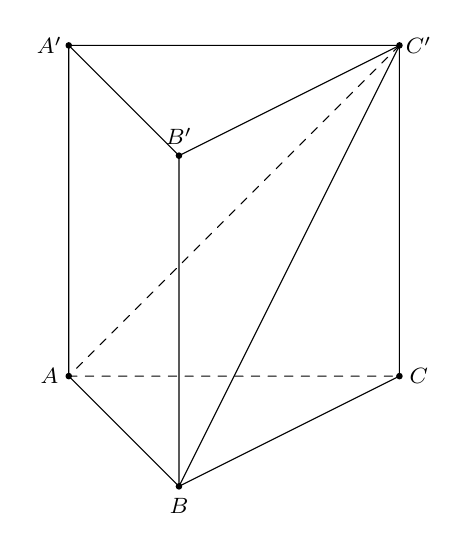
\begin{tikzpicture}[scale=0.7, font=\footnotesize, line join=round, line cap=round, >=stealth]
			\path
			(0,0)coordinate(A)
			(2,-2)coordinate(B)
			(6,0)coordinate(C)
			(0,6)coordinate(A')
			(2,4)coordinate(B')
			(6,6)coordinate(C')
			;
			\draw (A)--(B)--(C)--(C')--(B')--(A')--(A) (B')-- (A')--(C')--(B)--(B');
			\draw[dashed] (A)--(C) (C')--(A);
			\foreach \d/\g in {A'/180, B'/90, C'/0, A/180, B/-90, C/0}{
				\draw[fill=black](\d) circle (1.4pt) +(\g:.35)node{$\d$};}
			\end{tikzpicture}}
	}
\end{ex}

\begin{ex}%[Tô Ngọc Thy, PTDMH2023]%[2H1K3-2]
	Hình lăng trụ đứng $ABC.A'B'C'$ có diện tích đáy bằng $4$, diện tích ba mặt bên lần lượt là $9$, $18$ và $10$. Thể tích khối lăng trụ $ABC.A'B'C'$ bằng
	\choice
	{$\sqrt{11951}$}
	{\True $\dfrac{\sqrt{11951}}{2}$}
	{$\sqrt[4]{11951}$}
	{$\dfrac{\sqrt[4]{11951}}{2}$}
	\loigiai{
		\immini{Đặt $AA'=x$, $AB=c$, $AC=b$, $BC=a$.\\
			Ta có$\heva{&xc=18\\&xb=9\\&xa=10}\Rightarrow \heva{&c=2b\\&a=\frac{10}{9}b.}$\\
			Ta lại có $S_{ABC}=4\Leftrightarrow\sqrt{p\left(p-a\right)\left(p-b\right)\left(p-c\right)}=4$,\\
			với $p=\dfrac{a+b+c}{2}=\dfrac{37}{18}b$.\\
			$\Leftrightarrow\sqrt{\dfrac{37}{18}b\left(\dfrac{37}{18}b-\dfrac{10}{9}b\right)\left(\dfrac{37}{18}b-b\right)\left(\dfrac{37}{18}b-2b\right)}=4$.\\ 
			Suy ra $x=\dfrac{\sqrt{11951}}{8}$.\\
			Vậy thể tích khối lăng trụ \\
			$ABC.A'B'C'$ là $V=AA'\cdot S_{ABC}=\dfrac{\sqrt{11951}}{2}$.
			}
		{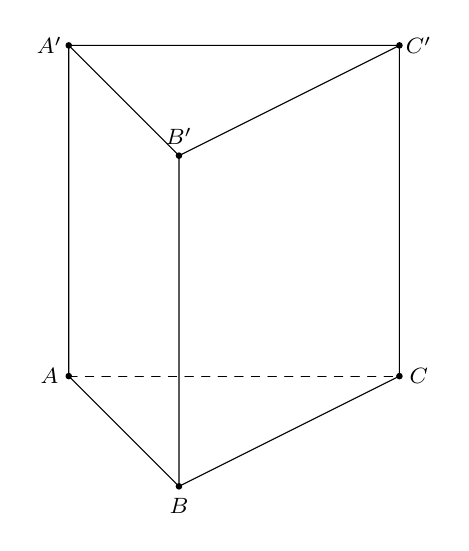
\begin{tikzpicture}[scale=0.7, font=\footnotesize, line join=round, line cap=round, >=stealth]
			\path
			(0,0)coordinate(A)
			(2,-2)coordinate(B)
			(6,0)coordinate(C)
			(0,6)coordinate(A')
			(2,4)coordinate(B')
			(6,6)coordinate(C')
			;
			\draw (A)--(B)--(C)--(C')--(B')--(A')--(A) (B')-- (A')--(C') (B)--(B');
			\draw[dashed] (A)--(C);
			\foreach \d/\g in {A'/180, B'/90, C'/0, A/180, B/-90, C/0}{
				\draw[fill=black](\d) circle (1.4pt) +(\g:.35)node{$\d$};}
			\end{tikzpicture}}
	}
\end{ex}

\begin{ex}%[Tô Ngọc Thy, PTDMH2023]%[2H1K3-2]
	Cho lăng trụ đứng $ABCD.A'B'C'D'$ có đáy là hình thang vuông tại $A$ và $B$, gọi $E$ là trung điểm $AD$. Cho $AD=2AB=2BC=2a$. Hãy tính theo $a$ thể tích khối lăng trụ $ABCD.A'B'C'D'$ biết khoảng cách giữa hai đường thẳng $BE$ và $A'D$ là $\dfrac{3\sqrt{22}}{22}a$.
	\choice
	{$9a^3$}
	{$\dfrac{9\sqrt{22}}{11}a^3$}
	{\True $\dfrac{9}{2}a^3$}
	{$\dfrac{9\sqrt{22}}{22}a^3$}
	\loigiai{
		\immini{Từ giả thiết, ta có tứ giác $ABCE$ là hình vuông.\\
			Hạ $AH\perp A'C$; $H\in A'C$.\\
			Ta có $CD\perp AC$, $CD\perp AA'\Rightarrow CD\perp (AA'C)$\\
			$\Rightarrow CD\perp AH$, mà $AH\perp A'C\Rightarrow AH\perp (A'CD)$.\\
			Mặt khác $BE\parallel CD$, $CD\in (A'CD)$,\\
			$E$ là trung điểm $AD$ nên\\ $\text{d}\left(BE;A'D\right)=\text{d}\left(E;(A'CD\right)=\dfrac{1}{2}\text{d}\left(A;(A'CD)\right)=\dfrac{1}{2}AH$.\\
			Từ giả thiết ta có	}
		{\begin{tikzpicture}[scale=0.7, font=\footnotesize, line join=round, line cap=round, >=stealth]
			\path
			(0,0)coordinate(A)
			(-1,-2)coordinate(B)
			(3,-2)coordinate(C)
			(8,0)coordinate(D)
			(0,6)coordinate(A')
			(-1,4)coordinate(B')
			(3,4)coordinate(C')
			(8,6)coordinate(D')
			(4,0)coordinate(E)
			($(A')!0.6!(C)$)coordinate(H)
			;
			\draw (D')--(A')--(B')--(C')--(D')--(D) (B)--(C)--(C') (B)--(B') (D)--(C);
			\draw[dashed] (H)--(A)--(A')--(C) (B)--(A)--(D)--(A') (B)--(E)--(C)--(A);
			\foreach \d/\g in {A'/90, B'/180, C'/90,D'/10, A/180, B/-90, C/-90,D/0,E/90,H/30}{
				\draw[fill=black](\d) circle (1.4pt) +(\g:.35)node{$\d$};}
			\draw
			pic[draw, angle radius=2mm]{right angle=A--H--A'};
			\end{tikzpicture}}
		\noindent
		$\dfrac{1}{2}AH=\dfrac{3\sqrt{22}}{22}a\Leftrightarrow AH=\dfrac{3\sqrt{22}}{11}a\Leftrightarrow\dfrac{AA'\cdot AC}{\sqrt{AA'^2+AC^2}}=\dfrac{3\sqrt{22}}{11}a\Leftrightarrow\dfrac{AA'\cdot a\sqrt{2}}{\sqrt{AA'^2+2a^2}}=\dfrac{3\sqrt{22}}{11}a\Leftrightarrow AA'^2=9a^2\Leftrightarrow AA'=3a$.\\			
		Ta có $S_{ABCD}=\dfrac{1}{2}(AD+BC)\cdot AB=\dfrac{1}{2}(2a+a)\cdot a=\dfrac{3a^2}{2}$.\\
		Vậy $V_{ABCD.A'B'C'D'}=S_{ABCD}\cdot AA'=\dfrac{3a^2}{2}\cdot 3a=\dfrac{9}{2}a^3$.
	}
\end{ex}

\Closesolutionfile{ans}
%======================
\subsection{Bảng đáp án}
\inputansbox{8}{ans/ANS-DANG-1}
